\let\TeXyear\year
\documentclass{ieeeaccess}
\let\setyear\year
\let\year\TeXyear

\usepackage{cite}
\usepackage{amsmath,amssymb,amsfonts}
\usepackage{algorithm,algorithmic}
\usepackage{graphicx}
\usepackage{textcomp}
\usepackage{caption}
\usepackage{helvet}  
\usepackage{comment}
\usepackage{pgfplots}
\usepackage{pgfplotstable}
\usepackage{listings}
\usepackage{booktabs}
\usepackage{siunitx}
\usepackage{setspace}
\usepackage{array}
\usepackage{multirow}


\newcolumntype{L}[1]{>{\raggedright\let\newline\\\arraybackslash\hspace{0pt}}m{#1}}
\newcolumntype{C}[1]{>{\centering\let\newline\\\arraybackslash\hspace{0pt}}m{#1}}
\newcolumntype{R}[1]{>{\raggedleft\let\newline\\\arraybackslash\hspace{0pt}}m{#1}}

\pgfplotsset{compat=1.7}
\setyear{2023}
\NewSpotColorSpace{PANTONE}
\AddSpotColor{PANTONE} {PANTONE3015C} {PANTONE\SpotSpace 3015\SpotSpace C} {1 0.3 0 0.2}
\SetPageColorSpace{PANTONE}

\newtheorem{Problem}{Problem}
\newtheorem{Definition}{Definition}

\def\BibTeX{{\rm B\kern-.05em{\sc i\kern-.025em b}\kern-.08em
    T\kern-.1667em\lower.7ex\hbox{E}\kern-.125emX}}

\captionsetup{font={sf,small,stretch=0.80},labelfont={bf,color=accessblue}}

\begin{document}
\history{Date of publication xxxx 00, 0000, date of current version xxxx 00, 0000.}
\doi{10.1109/ACCESS.2017.DOI}

\title{Semantic Maps for Knowledge Graphs: A Semantic-based Summarization Approach}
\author{
\uppercase{P. Camarillo-Ramirez} \authorrefmark{1},
\uppercase{F. Cervantes-Alvarez} \authorrefmark{1}, and
\uppercase{L. F. Guti\'{e}rrez-Preciado}\authorrefmark{1}}
\address[1]{Western Institute of Technology and Higher Education, Guadalajara, 45601 Mexico (pablo.camarillo@iteso.mx;fcervantes@iteso.mx;lgutierrez@iteso.mx;)}

\tfootnote{This work was supported in part by the  National Council
of Science and Technology of Mexico under Grant 498322}

\markboth
{P. Camarillo-Ramirez \headeretal: Semantic Maps for Knowledge Graphs: A Semantic-based Summarization Approach}
{P. Camarillo-Ramirez \headeretal: Semantic Maps for Knowledge Graphs: A Semantic-based Summarization Approach}

\corresp{Corresponding author: P. Camarillo-Ramirez (e-mail: pablo.camarillo@iteso.mx)}

\graphicspath{ {img/} }

\begin{abstract}
Knowledge Graphs (KGs) have emerged as a powerful
tool for representing semantic structured information
and enabling the development of intelligent systems.
This paper focuses on the generation of semantic maps 
as summarization method for KGs. We propose
a strategy that utilizes centroid-based clustering 
algorithms, namely Affinity Propagation and Partitioning
Around Medoids (PAM), to capture the semantic distance 
between nodes in the KG and generate meaningful 
clusters. Our experiments demonstrate divergent results 
between the two clustering algorithms, with Affinity
Propagation showing qualitative coherence and 
meaningfulness, while PAM performs well in terms of
internal validation metrics. We leverage the computed 
centroids to infer a main term of the semantic map, which contributes to the visually appealing and informative
representation of the KG. The combination of semantic 
distance capture, clustering algorithms, and centroid-based
inference facilitates a comprehensive understanding of the KG. Our findings highlight the importance of considering
both qualitative and quantitative evaluation measures in 
assessing clustering results. The effectiveness of semantic 
maps is showcased in visualizing KGs and advancing the
field of knowledge graph visualization. The integration of
centroid-based clustering algorithms, qualitative evaluation,
and inference methods offers improved clarity and 
interpretability for complex KG analysis.
\end{abstract}

\begin{keywords}
Knowledge graphs; Knowledge graph visualization; Semantic distance; Semantic mapping; Visual data exploration; Clustering
\end{keywords}

\titlepgskip=-15pt

\maketitle

\section{Introduction}
\label{sec:introduction}
Knowledge Graphs are considered as the fundamental 
building blocks for AI systems, providing the necessary
foundation for representation and reasoning capabilities
to address the imperative design requirement of involving
humanity in the loop \cite{Purohit2020}. The idea behind
a Knowledge Graph (KG) is to represent knowledge from
real world in a graph structure, where nodes represent 
entities of interest and edges represent relations between 
these entities \cite{Hogan21}. Recently, academic and 
private organizations have constructed KGs, such as  YAGO 
\cite{suchanek2007yago}, DBPedia \cite{auer2007dbpedia}, 
Freebase \cite{Freebase08}, NELL\cite{NELL10}, Google 
Knowledge Graph \cite{GoogleKG12}, Microsoft Satori 
\cite{Satori13}, Facebook Entity Graph \cite{Facebook13}, 
and Wikidata \cite{Wikidata14}, which contain millions of entities and billions of relationships. The main applications
of KGs include the enhancement of search engines like 
Google \cite{GoogleKG12} or Bing \cite{Satori13}, question 
answering \cite{Chen2022}, information retrieval, 
recommender systems \cite{Lin2022, Haotian2022}, domain
specific KG building \cite{Zhang2022, Borrego2022, Guan2022},
and decision support in the life sciences
\cite{Zou_2020,Belleau08,Ruttenberg09,Momtchev09}.

Considering the continuous increase in the use of 
KGs in decision-making applications, it becomes 
important to compress and summarize KGs for efficient
representation of data \cite{gunaratna2017}. In 
general, one of the applications of summarizing
graphs is to reduce the data volume and storage
to facilitate the process of graph visualization
\cite{liu2018graph}. Visual data exploration is
considered as a hypothesis-generator process by
allowing users to gain a deep understanding of 
the data \cite{keim2001visual}, hence summarizing
a KG is crucial to produce an effective visual 
representation to understand relationships 
between entities and concepts in a domain. By
representing the information in a visual format, 
users can quickly identify patterns, trends, and
clusters or related information that may be 
difficult to see in a text-based representation. 
Existing approaches to visualize KGs are focussed on 
drawing the whole structure \cite{gomez2018visualizing} 
preventing data analysts to explore the KG beyond its 
structural information.

Semantic maps, on the other hand, are widely used 
technique to understand complex topics 
\cite{SemanticMaps19}. They involved 
a categorical structuring of information in a
graphic form \cite{johnson1986semantic}. A semantic map
typically has a central word that represents the main
topic, connected to a set of keywords that
groups the remaining vocabulary. Generating a
a semantic map requires identifying groups of 
related words. Unsupervised learning provides 
clustering algorithms that classify data into one or 
more classes based on similarity or distance 
measures \cite{SCHAEFFER200727}. In theory, applying
a clustering strategy to the vocabulary in a KG will
result in groups that can be used to construct the 
semantic map. Section \ref{sec:results} presents a set of 
experiments validating the above notion.

The main contribution of this work is to provide 
a novel approach for summarizing KGs by leveraging
the power of semantic maps. Some KG applications, 
such as query answering or KG visualization, 
require reduced versions of the original graphs \cite{gomez2018visualizing,Jalota2021}. To address
this challenge, we propose a method that generates 
a reduced version of a KG by creating semantic maps
from the knowledge graph, enabling users to 
explore and comprehend the underlying structure and 
relationships of the graph in a visually intuitive manner. 
In addition, we present a formal definition of the semantic 
map of a KG and propose a strategy to measure the quality
of these semantic maps. To demonstrate the utility of these
semantic maps in providing a high-level view of a KG, we 
conduct a survey on a group of experts that compared the use
of semantic maps with the classical visual representation 
of KGs. These experiments showcase
the value of semantic maps in offering a comprehensive 
understanding of the KG's structure and relationships.

%In this paper, we 
%hypothesize that semantics maps are useful to visualize
%the high level of abstraction of a KG based on the 
%semantic closeness of entities in the KG.

The paper is structured as follows. Section \ref{sec:KG} 
provides details on KGs and establishes a definition that
will be used throughout the rest of the paper. In Section \ref{sec:related}, we review the most relevant 
literature related to knowledge graph 
visualization, graph clustering, semantic similarly,
and semantic mapping topics. Section \ref{sec:Method},
describes the proposed method and the algorithms necessary
for generating semantic maps of a KG. In Section 
\ref{sec:results}, we discuss the results obtained from
a series of experiments evaluating the method of 
generating semantic maps generated from a collection
of datasets extracted from DBPedia. Finally, Section 
\ref{sec:conclusions} presents concluding remarks and 
outlines future work.

\section{Foundations of Knowledge Graphs}
\label{sec:KG}

Some definitions describe a KG as a graph-structured
knowledge base \cite{nickel2015review, 
seufert2016instant}. In this work, we consider a
knowledge base a set of sentences/facts expressed in
some formal language such as description logic. In 
other words, KGs consist in a collection of facts 
formed by \texttt{<subject,predicate,object>}. These
collections are typically represented in languages, 
such as RDF (Resource Description Framework) \cite{RDF},
OWL (Ontology Web Language) \cite{OWL}, or N-Triples 
which is a subset of the more complex RDF/XML syntax,
is designed to be both human-readable and 
machine-readable. It is a plain text format that 
represents RDF statements using 
subject-predicate-object triples, with
each element separated by white space and terminated
by a period.

In the field of computer science, an ontology serves as a 
descriptive model of the world, comprising a collection of
types, properties, and relationship types 
\cite{Garshol2004MetadataTT}. According to description logic 
terminology, knowledge bases have two types of axioms: a 
terminology box (TBox) and an assertion box (ABox) 
\cite{horrocks2008ontologies}, hence a KG should contain
these two sets of axioms to be considered as a knowledge base.
To exemplify the above idea, Figure \ref{Fig:TboxAndAbox} 
shows sets TBox and ABox of a group of entities and 
relationships extracted from DBPedia \cite{auer2007dbpedia} 
\footnote{https://dbpedia.org (Last visited: 2023-11-16)}. In 
KGs, the ontology classes (e.g.,\texttt{dbo:Book} 
\footnote{URIs mentioned in this document use the 
common prefixes described in https://prefix.cc} or 
\texttt{dbo:Movie}) correspond with the TBox and 
describe concepts hierarchies, while the ontology 
instances correspond with the ABox and describe entity 
instances (e.g.,\texttt{dbr:Lucasfilm} or 
\texttt{dbr:George\_RR\_Martin}) and their
relationships. Hierarchical relationships like 
\textit{"is a"} defines the connection between each 
pair of concepts in TBox. For example, axioms 
(\texttt{dbo:Book}, \textit{is a}, 
\texttt{dbo:Work}) and (\texttt{dbo:film},
\textit{is a}, 
\texttt{dbo:Work}) describe the fact that both 
\texttt{dbo:Book} 
and \texttt{dbo:film} concepts are descendants of the 
class
\texttt{dbo:Work}. Alternatively, in ABox, axioms also
indicate the list of types that one entity instance may
have. For instance, in Figure \ref{Fig:TboxAndAbox}, 
the axiom (\texttt{dbr:A\_dance\_of\_dragons}, 
\textit{rdf:type},
\texttt{dbo:Book}) indicates that resource
\texttt{dbr:A\_dance\_of\_dragons} is an instance
of class
\texttt{dbo:Book}. Another type of axioms in ABox like
(\texttt{dbr:George\_RR\_Martin}, is 
\textit{dbo:creator\_of}
of, \texttt{dbr:DaenerysTargaryen}) and 
(\texttt{dbr:George\_RR\_Martin}, is 
\textit{dbo:author} of,
\texttt{dbr:A\_dance\_of\_dragons}) indicate
that the instance \texttt{dbr:George\_RR\_Martin} has 
two semantic connections with 
\texttt{dbr:DaenerysTargaryen} and 
\texttt{dbr:A\_dance\_of\_dragons} entity instances.

\Figure[h!](topskip=0pt, botskip=0pt, midskip=0pt)
[width=0.95\textwidth]{img/TBoxAndAbox.pdf}
{Small group of concepts and instances extracted from 
DBPedia. \label{Fig:TboxAndAbox}}

Let us begin by proposing a formal definition
of a KG before proceeding to describe the 
remaining relevant topics associated 
with the semantic mapping process outlined in 
this paper.

\begin{Definition}[Knowledge Graph]
Let $V$ the set of entities, where each entity 
$v \in V$ can be uniquely identified. Let $L$ denote
the set of property labels or attributes associated 
with the entities in the knowledge graph. Each label 
$l \in L$ represents a specific property or 
characteristic of an entity. Let $E$ the set of edges
in a Knowledge Graph $K$. A knowledge graph $K$ is defined
as $K = (V, L, E)$, where $E$ is a subset of the cross
product of entities and property labels defined as 
$V \times L \times V$. Each member of $E$ is referred 
to as a triple $(subject-property-value)$.
\end{Definition}

From the definition above, we can deduce that a KG
can be represented as a list of triples that capture 
axioms from ABox or TBox. In this work, our focus lies
on the triples that represent axioms of the ABox set. 
Specifically, whenever an entity instance is mentioned, 
it is associated with the subjects of the ABox triples.

\section{Related work}
\label{sec:related}

In this section, we present a comprehensive overview 
of key topics that are fundamental to the understanding
and analysis of semantic maps of knowledge graphs. We 
begin by discussing some knowledge graph summarization approaches, 
which aim to distill large-scale graphs into concise 
and meaningful summaries, aiding in knowledge 
extraction and decision-making processes. Additionally, 
we explore the concept of semantic maps, which provide 
a visual depiction of the relationships and 
interdependencies among entities in a knowledge graph. 
We further examine semantic similarity measures, which 
quantify the relatedness between entities based on 
their semantic attributes or contextual information. 
We then go through centroid-based clustering 
algorithms, which leverage the concept of centroids to 
group similar entities within knowledge graphs. Lastly, 
we describe the significance of visual data 
exploration techniques on knowledge graphs and how semantic
maps of knowledge graphs can be .

\subsection{Knowledge Graph summarization}

In the context of data mining, summarization is the
process of facilitating the identification of 
meaningful data. The applications of graph 
summarization include reduction of data
volume and storage, speedup of graph algorithms and 
queries, interactive analysis support, and noise 
elimination \cite{liu2018graph}. Recently, it
has been proposed to summarize large graphs in order 
to enable an efficient visualization of their content. 
For example, in \cite{Koutra2019}, the authors focus 
on summarizing KGs by taking advantage of individual 
interests to generate personalized knowledge graph
summaries. In \cite{OntoVis}, Shen et al. propose a 
visual analytics tool called OntoVis, which performs 
both structural and semantic abstractions to offer a 
summarized version of a large graph and thus
being able to visualize a simplified version of the 
graph. Another related work is presented in 
\cite{koutra2014vog}, which describes the VoG
(Vocabulary-based summarization of Graphs) algorithm 
to summarize and understand large graphs by 
constructing and visualizing subgraph-types, 
such as starts, cliques, and chains. The visual 
abstraction presented in \cite{8801911}, transforms
geo-tagged social media data into high-dimensional
vectors by utilizing a doc2vec model.

Every summarization strategy 
depends on selecting an interest criteria to extract 
meaningful information \cite{liu2018graph}. However, 
to achieve a concise definition of \textit{interesting} 
is not an easy task. For example, the FUSE algorithm 
\cite {Seah12} proposes a profit maximization
model that seeks to find a summary by maximizing 
information profit under a budget constraint. On the
other hand, VoG \cite{koutra2014vog} exploits
the Minimum Description Length (MDL) principle aimed at 
identifying the best subgraphs by choosing those which 
save most bits. In the case of semantic abstraction
proposed in \cite{8801911}, a dual-objective blue 
noise sampling model is utilized to select a subset of
social media data items supporting the spatial 
distribution and semantic correlation for the resulting
simplified geographical visualization. The personalized 
summaries of KGs described in \cite{Koutra2019}, the 
criteria to decide which information is 
\textit{interesting} for each user is determined by
reviewing the users' query history. The work of M. 
Tasnmin et al. propose a strategy to find equivalent 
entities in a KG using the context of each RDF Molecule
\cite{Tasnim2020}. In terms of summary quality,
Riondato et al. \cite{Riondato2014} have proposed 
two quality metrics ($\ell_{p}$-reconstruction 
error and cut-norm error) primarily focused on 
determining the error generated in the adjacency
matrix from summarized graph. However, these metrics
have not been proven with summarization techniques
associated with KGs. The semantic
mapping process  described in this document can be
perceived as a summarization strategy that is aimed
at minimizing the semantic distance between each 
pair of entity instances in the KG as the criterion of 
interest.

\subsection{Semantic maps}
A semantic map is a type of graphical representation 
that shows the relationships between different concepts 
or words within a particular domain or field of study
\cite{johnson1986semantic}. The  purpose of a semantic 
map is to visually organize and display the meaning and 
connections between various terms or concepts, 
highlighting their semantic similarities and 
differences. In other words, a semantic map provides a 
visual representation of how different ideas or 
concepts are related to each other and how they are
grouped together based on their shared meanings or 
semantic properties. However, there are another mathematical
representations for semantic maps such as graph and 
Euclidean space \cite{Croft2022}. Figure  
\ref{fig:example_semantic_map} shows an
example of a semantic map describing the topic 
\textit{Water}. It contains three node categories: (1) 
the central word (root), (2) the set of keywords 
(e.g., Usages, Living things, etc.), and (3) the
vocabulary associated with each keyword, for instance, 
words \texttt{Cooking} and \texttt{Bathing} are 
associated with keyword \textit{Usages}.

\Figure[h]()[scale=0.35]{img/Water_Semantic_Map_no_colour.pdf}
{Example of a semantic map of concepts and vocabulary  associated with
topics \textit{Water}.\label{fig:example_semantic_map}}

\begin{Definition}[Semantic Map]
Let $C$ the set of groups of related words in the
vocabulary, $C_{i}$ the $i-th$ group of related
words, $kw$ the set of keywords representing
each group of related words, and $\alpha$ the
main subject of the vocabulary. Let us define 
a semantic map as a tree $T = (\alpha, E_{T}$), 
where $\alpha$ represents the root of this tree,
and $E_{T}$ contains the set of edges that
connects all nodes of the semantic map. 
$E_{T}$ is defined as follows: 
$E_{T} = (E_{kw} \cup E_{w})$, where
$E_{kw} = (\alpha \times kw)$, and $E_{w} = (kw_{i} \times w_{i}) 
\forall_{kw_{i} \in k}, \forall_{w_{i} \in C_{i}}$.
\end{Definition}

\subsection{Semantic similarity}

The semantic similarity is a metric used in Natural 
Processing Language (NPL) and Information Retrieval
(IR) areas \cite{HOVY20132} that represents how related 
are two concepts based on their hierarchical relations 
\cite{resnik1995using}, \cite{turney2010frequency}. 
In a KG, the semantic similarity between two 
entities $e_{1}, e_{2} \in V$ is denoted as $sim(e_{1}, e_{2})$. 
Intuitively, semantic distance between two words is the
most easy way to calculate semantic similarity and it is usually
determined by the path connecting two entities in KG. Existing
semantic similarities metrics are classified in two main 
groups: corpus-based and knowledge-based approaches 
\cite{mihalcea2006corpus}. Corpus-based 
similarity metrics are focused on learning how similar
are two concepts based on the information from large corpora.
Two examples of corpus-based similarity metrics are pointwise 
mutual information \cite{church1990word}, and latent semantic
analysis \cite{landauer1997solution}. In contrast, knowledge-based
similarity metrics quantify the degree to which two words are 
semantically related \cite{budanitsky2001semantic}. In KG, 
knowledge-based approaches, semantic similarity is determined
using the information provided by the TBox. Knowledge-based
approaches include path-based metrics such as those proposed 
by Hulpus et at. \cite{hulpucs2015path}, Wu and Palmer
\cite{wu1994verb}, and Leacock and Chodorow 
\cite{leacock1998combining}. Other knowledge-based measures
utilize the Information Content (IC) metric like Lin 
\cite{lin1998information}, Jiang and Conrath 
\cite{jiang1997semantic}, and Resnik \cite{resnik1995using}
metrics. IC of concepts is a statistical measure that computes
the specificity of a concept over a corpus. Higher 
values of IC indicate more specific concepts (e.g.,
\texttt{dbo:Book}) and lower values of IC are associated
with more general concepts (e.g., \texttt{owl:Thing}).
Hybrid knowledge-based approaches like IC-graph 
\cite{ZhuIglesias2017} or Zhou \cite{zhou2008new} combine
IC and some other metrics to compute how related two words
are. For instance, graph-based IC \cite{ZhuIglesias2017} 
uses a SPARQL query on DBPedia to compute $freq_{graph}(c_{i})$
and $N$ values in the following expression:

\begin{equation}
    \label{eq:ic_graph}
    IC_{graph}(c_{i}) = -logProb(c_{i})
\end{equation}

Where $Prob(c_{i}) = \frac{freq_{graph}(c_{i})}{N}$ and $N$ is the 
number of entities in the KG. Let $\mathcal{E}(c_{i})$ the set of 
entities having as type the concept $c_{i}$, the frequency of
concept $c_{i}$ in the $KG$ is defined as 
$freq_{graph}(c_{i}) = |\mathcal{E}(c_{i})|$.

\subsection{Centroid-based Clustering}

There exist several techniques to clustering 
data and recent surveys summarize these clustering
approaches based on the application or the type
of data to group \cite{Dongkuan2015}, 
\cite{DBLP:books/crc/aggarwal2013}, 
\cite{firdaus2015survey}. Types of clustering include
Centroid-based, Density-based, Distribution-based, and
Hierarchical clustering \cite{google_2022}. 

One of the phases of the semantic mapping process
is to collocate each entity into the most appropiate
cluster based on its semantic similarity. Each 
resulting cluster needs a node that represents all 
entities contained on it. We denote the set of this
representing nodes as the keywords of the semantic map. 
Considering these keywords as centroids of clusters, 
the usage of a centroid-based clustering is crucial.

The main idea of centroid-based clustering is to find 
\textit{k} centroids (or centers) followed by computing
\textit{k} sets of data points that minimize the proximity
with each center. For instance, K-means algorithm tries
to minimize the sim of the squared distance between the 
data points and the cluster's centroid
\cite{McQueen67}. A variation of K-means
is the PAM (Partitioning Around Medoids) algorithm that
minimizes dissimilarities between points in a cluster 
and the centroids  \cite{kaufmanPAM}. The CLARA 
(Clustering Large Applications) algorithm is 
an extension of PAM for large datasets \cite{kaufmanCLARA}.
On the other hand, CLARANS (Clustering Large 
Applications based on RANdomized Search) is a partitioning
algorithm focused on spatial data mining because it recognizes
patterns and relationships existing in spatial data such as 
topological data \cite{ng2002clarans}. One last centroid-based
clustering algorithm is the Affinity Propagation (AP) 
algorithm which consists on a message-passing procedure
that looks for broadcasting messages of attractiveness and 
availability among data points \cite{frey2007clustering}.

\subsection{Cluster quality}

Literature offers two classes of clustering validation
measures: external  clustering validation and internal
clustering validation \cite{DBLP:books/crc/aggarwal2013}. 
Internal validation metrics evaluate the quality of a 
clustering algorithm based on its intrinsic 
properties, while external validation methods evaluate
the quality of a clustering solution based on its agreement
with a known label of the data. Since there is no known
label of the datasets used in the experiments described
in this work, our proposal is to use internal validation
measures such as Silhouette score \cite{kaufmanPAM}, 
Davies-Bouldin score \cite{davies1979cluster}, 
and Calinski-Harabasz Index \cite{calinski1974dendrite}.

Each internal validation metric measure different aspects
of the clusters. For example, Silhouette score measures
how well each data point fits into its assigned cluster 
compared to other clusters \cite{kaufmanPAM}. Inertia of 
a cluster, also known as the within-cluster sum of squares
(WSS) metric measures how tightly packed the data points
are within each cluster \cite{McQueen67}. The goal is to
minimize inertia, 
which is equivalent to maximizing the distances between
clusters. On the other hand, Dunn index measures the distance between the nearest points in different clusters and the
distance between the farthest points in each cluster 
\cite{dunn1974well}. Another known quality measure is 
the Davies-Bouldin index which measures the similarity 
between each cluster and its closest neighboring cluster,
while also considering the cluster's internal similarity 
\cite{davies1979cluster}. Finally, Calinski-Harabasz 
index measures the ratio of between-cluster variance 
to within-cluster variance \cite{calinski1974dendrite}.

\subsection{Visual Data Exploration of knowledge graphs}

The idea behind the visual data exploration 
process is to present the data in some visual 
form, allowing users to draw conclusions from
the analyzed phenomena \cite{keim2001visual}. 
This process, also known as the \textit{information 
seeking mantra}, follows three steps: overview,
zoom and filter, and details-on-demand 
\cite{Shneiderman96}. In this context, the visual
representation of KGs offered by semantic maps 
proposed in this paper, provides a new way to 
visualize KGs. It does so by emphasizing the 
semantic closeness of their entity nodes. Recent
works \cite{6787141,1703364,8801911} have shown that
visualizing a simplified version of a large graph
is an adequate alternative.

In regard to visual exploration of KGs, challenges
include context adaptation, users input 
\cite{Koutra2019}, data heterogeneity
\cite{OntoVis,6787141,1703364}, supporting diverse 
analysis tasks (query, combination, filtering, etc.), 
and performance \cite{gomez2018visualizing}. In this
study, semantic mapping proposal is to combine and 
reduce the number of edges in the KG using the 
semantic similarity among its entities to compute 
clusters of related entities.

Recent applications have proven useful for large graph
visualizations to understand different phenomena, such
as Bitcoin transactions \cite{mcginn2016visualizing} 
and online discussions \cite{molina2017improving}. For
big knowledge graphs, it is necessary a distributed 
implementation of the layout algorithms to improve the 
time needed to generate the visual representation
\cite{gomez2018visualizing}. Actually, Consalvi et. al 
\cite{Consalvi2022} propose a self-contained system to 
compute interactive visualizations of thousands 
elements in a mobile browser.

In addition of recent efforts on KGs visualization, 
there are some commercial products enabling analysts to 
visualize RDF graphs like Data 
Graphs\footnote{https://datagraphs.com (Last visited: 2023-11-16)} or the 
family of tools developed by Cambridge Intelligence 
company: Keylines, ReGraph, and KronoGraph 
\footnote{https://cambridge-intelligence.com/ (Last visited: 2023-11-16)}
that offer the capability to render KGs to support 
tasks in areas like pharmacy and bio-science research 
or financial analysis. In the area of 
free tools, there are two online tools that consumes 
RDF data and produce a visual representation: RDF 
visualizer \footnote{https://issemantic.net/rdf-
visualizer (Last visited: 2023-11-16)} and RDF grapher 
\footnote{https://www.ldf.fi/service/rdf-grapher (Last visited: 2023-11-16)}. The
main limitation with these tools is the small amount 
of data they can process.
\section{Proposed method}
\label{sec:Method}

\Figure[h!](topskip=0pt, botskip=0pt, midskip=0pt)[width=1\textwidth]{img/origin.pdf}
{Visual representation from a small KG containing some fictional characters by George R.R. Martin. a) Contains the visual representation produced by the online RDF visualizer. b) Inferred semantic map of the original KG.\label{Fig:DefaultVisualization}}

\Figure[h!](topskip=0pt, botskip=0pt, midskip=0pt)[width=0.95\textwidth]
{img/semantic_mapping_process.pdf}
{Semantic mapping phases. 
(a) Consume a KG as a list of n-triples, 
(b) Generate the semantic distance matrix $D$,
(c) Cluster entities using the matrix $D$,
(d) Infer main term $\alpha$, and
(e) Assemble the semantic map by connecting each centroid with $\alpha$.
\label{fig:Semaf}}

The notion behind the semantic map of a KG is 
to produce a reduced version of the KG by 
exploiting the semantic similarity between each
pair of entities. To illustrate this idea, let us 
generate a small KG from DBPedia containing the 
list of some fictional characters from series of
fantasy novels by the novelist George R. R. Martin.
Figure \ref{Fig:DefaultVisualization}a) presents 
a visual representation produced by the online
RDF graph visualizer 
\footnote{https://issemantic.net/rdf-visualizer (Last visited: 2023-11-16)}, 
which is an online tool that allows easy to visualization
and analysis RDF datasets.
However, this kind of visualization is not visually
informative or visually appealing which may lead 
in an ineffective exploratory visual analysis. 
Contrarily Figure \ref{Fig:DefaultVisualization}b)
exhibits a semantic map of the KG. This semantic map uses
a node-link representation to display the set of entity
instances of the KG connected with their corresponding
centroid and all centroids connected with the central
concept of the semantic map.


\subsection{Extracting semantic distance of entities in a
Knowledge Graphs}

The first phase of the semantic mapping process is to
group the entities of the KG based on the semantic 
closeness between each pair of entities in the KG. 
The main challenge in this phase is to extract 
numeric data from the KG and generate a set of
entity group. We propose computing the semantic
distance for each pair of entities in the KG by
generating a semantic distance matrix.

\begin{Definition}[Semantic distance matrix]
Given a Knowledge Graph $K = (V, L, E)$, and 
$sim(e_{1}, e_{2})$ the semantic similarity between
entity instances $e_{1}$ and $e_{2}$, the semantic 
similarity matrix $D(K)$ represents the semantic 
distance between each pair of entity instances in $E$.
Specifically, the value for cell $d_{i,j} = 1 - 
sim(e_{i}, e_{j})$.
\end{Definition}

Algorithm \ref{alg:matrix} describes the process to 
compute the distance semantic matrix $D$. The algorithm 
begins by generating the set of triples that represent 
the KG from the set of edges $E$. For each edge $e \in E$,
the subject, property label, and target
entity instance are extracted using the functions 
$subject()$, $property()$, and $value()$, respectively. 
Subsequently, for each pair of triples $t_{i}, t_{j} \in T$,
the semantic similarity is computed using the $sim()$. 

\begin{algorithm}
 \caption{Algorithm to build the semantic distance matrix}
 \label{alg:matrix}
 \begin{algorithmic}[1]
 \renewcommand{\algorithmicrequire}{\textbf{Input:}}
 \renewcommand{\algorithmicensure}{\textbf{Output:}}
 \REQUIRE Set of edges $E$ of K
 \ENSURE  Semantic distance matrix $D$
  \STATE $T = \emptyset$
  \FORALL{$e \in E$}
    \STATE $T = T \bigcup \{(subject(e), property(e), value(e))\}$ 
  \ENDFOR
  \FORALL {($t_{i}, t_{j}) \in T \times T$}
    \IF{$t_{i} = t_{j}$}
        \STATE $D(i, j) = 0$
    \ELSE
        \STATE $e_{a} = subject(t_{i})$
        \STATE $e_{b} = subject(t_{j})$
        \STATE $D(i,j) = D(j, i) = 1 - sim(e_{a}, e_{b})$
    \ENDIF
  \ENDFOR
 \RETURN $D$ 
 \end{algorithmic} 
 \end{algorithm}
 

The computational complexity of the function $sim()$
is not detailed by original authors in \cite{ZHU201730}, 
however, we can provide a brief discussion on the 
computational complexity based on the provided 
description of the algorithm and the available
code of $sim()$ 
\footnote{https://github.com/gsi-upm/sematch (Last visited: 2023-11-16)}.
The function $sim()$ receives as input parameters
the reference of two entities in the YAGO KG, let's
call them $e_{1}$ and $e_{2}$. It consists of 
five phases:

\begin{enumerate}
    \item Extracting concepts from the YAGO KG,
    \item Mapping concepts to synsets,
    \item Calculating the IC metric,
    \item Calculating scores for synsets, and
    \item Obtaining the final score for the given entities.
\end{enumerate}

The filtering step takes linear time, specifically 
$O(N_{1} + N_{2})$, where $N_{1}$ and $N_{2}$ 
represent the number of concepts associated with 
entities $e_{1}$ and $e_{2}$, respectively. Similarly,
mapping concepts to synsets for each entity takes linear
time, $O(N_{1} + N_{2})$, for each entity. Calculating 
the IC for each synset and finding the most common 
synsets also takes linear time, $O(N_{1} + N_{2})$. 
The comparison and score calculation involve nested
loops. In the worst case, there are $N_{1}$ iterations
for the score of $e_{1}$ and $N_{2}$ iterations for
the score of entity $e_{2}$. This results in a time
complexity of $O(N_{1} \cdot N_{2})$. The final score
calculation is a constant-time operation, $O(1)$. 
Overall, the most time-consuming part of the code is 
the nested loop for comparing synsets and calculating
scores, which results in a time complexity of 
$O(N_{1} \cdot N_{2})$.


The relation between similarity and distance follows 
the notion that the higher is the similarity between 
two entities the lower is the distance between these 
entities. The $i-th$ row of $D(K)$ is the vector 
containing semantic distance values between the $i-th$
entity and the rest of entities in the KG. The semantic
distance between each entity and itself is $0$. Our 
proposal consist of using a centroid-based clustering 
algorithm and generate a non-overlapping
set of clusters by using the semantic distance matrix
$D$ as input of the selected clustering algorithm. 

\subsection{Clustering entities of Knowledge Graphs}

One of the central needs of semantic maps is
to find specific nodes in the KG that represent
each group of entity instances. Center-based 
clustering algorithms seem to be suitable for
this purpose.
We propose using PAM and Affinity Propagation 
center-based clustering algorithms due to their 
compatibility with handling distance matrices 
as input instead of feature vectors \cite{kaufmanPAM,
frey2007clustering}. PAM is a clustering algorithm
that works by iteratively selecting a set of 
$k$ medoids from the data points and assigning 
each non-medoid point to
its closest medoid. The algorithm tries to minimize
the sum of distances between each data point and
its assigned medoid. On the other hand, Affinity 
Propagation is a clustering algorithm that works 
by propagating messages between data points to 
determine which points should be exemplars
(i.e., representatives of their clusters). 

Let $C = \bigcup C_{i}$ the set of clusters 
resulting after applying a centroid-based clustering
algorithm. Each cluster $C_{i}$ has a centroid element
denoted by $centroid(C_{i})$ and the set of centroid
elements is defined in the Equation \ref{eq:set_of_centroids}.

\begin{equation}
    \label{eq:set_of_centroids}
   \mu = \bigcup_{C_{i} \in C} centroid(C_{i}). 
\end{equation}

\subsection{Central concept of the semantic map}

One of the main features of a semantic map is the
\textbf{central concept} that represents the main 
topic of this graphical representation. In this work,
we denote this central concept as $\alpha$. In a 
regular semantic map, $\alpha$ is connected with
a set of selected keywords (e.g., {structures,
characteristics, size, habitat, movie, kinds} in 
Figure \ref{fig:example_semantic_map}). These 
keywords are used to represent every group of 
words of the semantic map. This work proposes to
use the centroids inferred by centroid-based clustering 
algorithms \cite{Dongkuan2015} as the keywords
of a KG. Therefore, we denote these keywords as
the set of centroids $\mu$ of the entities in a KG,
where each $\mu_{i}$ represents the centroid of
i-th cluster $C_{i}$, i.e., 
$\mu_{i} = centroid(C_{i})$.

To infer the central term $\alpha$, we propose to
compute the $IC_{graph}$ measure for all types 
associated with each centroid in $\mu$. Let 
$types(e_{i})$ to be the function to retrieves
set of types associated with the entity $e_{i}$, 
we define $\mathcal{T}$ as the set of shared types
among all centroids in $\mu$ This definition is formally
described in equation \ref{eq:shared_types}.

\begin{equation}
    \label{eq:shared_types}
    \mathcal{T} = \bigcap_{\mu_{i} \in \mu} types(\mu_{i})
\end{equation}

\begin{Definition}[Central concept $\alpha$]
Given a set of shared types 
$\mathcal{T}$, the central concept $\alpha$ of $K$ is the concept
$c_{i} \in \mathcal{T}$ with maximum $IC_{graph}$.
\end{Definition}

\begin{algorithm}
\caption{Algorithm to infer main term $\alpha$ of $K$}
\label{alg:infer_alpha}
\begin{algorithmic}[1]
\renewcommand{\algorithmicrequire}{\textbf{Input:}}
\renewcommand{\algorithmicensure}{\textbf{Output:}}
\REQUIRE $\mu$: Set of centroids of $C$.
\ENSURE $\alpha$: Main term of $K$
\STATE $\mathcal{T} = types(\mu_{0})$ 
\FORALL{$\mu_{i} \in \mu - \mu_{0}$}
    \STATE $\mathcal{T}$ = $\mathcal{T} \cap types(\mu_{i})$ 
\ENDFOR
\STATE $\alpha = max(IC_{graph}(\mathcal{T}))$
\RETURN $\alpha$
\end{algorithmic} 
\end{algorithm}

Algorithm \ref{alg:infer_alpha} formalizes the 
process of inferring the main term of $K$ by 
initializing the set of shared types, denoted
as $\mathcal{T}$, with the types associated with
the centroid of cluster $C_{0}$. The computational
complexity of $IC_{graph}()$ (See eq. \ref{eq:ic_graph})
depends on the complexity of building the set
of entities having as type the concept 
$c_{i}$, denoted as $\mathcal{E}(c_{i})$. To 
achieve this, we need to traverse the entire KG,
which has a time complexity of $O(N)$, 
where $N$ is the number of nodes in the KG. 
For each node, we must retrieve the list of types
and search for the concept $c_{i}$. Assuming that
the complexity of obtaining the list of types is
$O(t)$, where $t$ is the number of types 
associated with concept $c_{i}$, the overall
complexity of $IC_{graph}()$ is $O(N \cdot t)$.


\subsection{Semantic map of a Knowledge Graph}

Let us define the semantic map of a KG:

\begin{Definition}[Semantic map of a Knowledge Graph]
Given a Knowledge Graph $K = (V, L, E)$, a semantic
distance matrix $D(K)$, the main term of $K$: $\alpha$, 
the semantic map of $K$ is defined as $\mathcal{SM}(K) 
= (\alpha, E_{K})$.
\end{Definition}

Table \ref{tab:symbols}
describes the symbols associated with semantic maps 
of KGs.

\begin{table}[!htb]
\caption{Symbols associated with semantic maps of 
Knowledge Graphs.}
\label{tab:symbols}
\centering
\begin{tabular}{lL{6.5cm}}
     \toprule
     \textbf{Symbol} & 
     \textbf{Description} 
     \\
     \midrule
     $\alpha$ & Main concept of the semantic map. \\
     \hline
     $\mu$ & Set of centroid entities produced by a 
     centroid-based clustering algorithm, where 
     $\mu \subseteq V$. \\
     \hline
     $C$ & Set of clusters resulting from running a 
     centroid-based algorithm. \\
     \hline
     $\mathcal{NC}$ & Non-centroids entities in KG, where
     $\mathcal{NC} \subseteq V$ and $\mathcal{NC} \cap \mu = 
     \emptyset$.\\
     \hline
     $E_{nc}$ & Set of edges connecting all members of the
     clusters with their corresponsing centroid, defined as 
     $\mu_{i} \times x, \forall x \in \mathcal{NC}$ and $\forall \mu_{i} 
     \in \mu$. \\
     \hline
     $E_{\mu}$ & Set of edges connecting all centroids with
     the main term $\alpha$, definded as $E_{\mu} = 
     \mu_{i} \times \alpha, \forall \mu_{i} 
     \in \mu$.
     \\
     \hline
     $E_{K}$ & Set of edges connecting each all elements in the semantic map, 
     defined as $E_{K} = E_{\mu} \bigcup E_{nc}$. \\
     \bottomrule
\end{tabular}
\end{table}

Semantic mapping process aggregates the process of 
clustering entities of KG and inferring the central 
term $\alpha$. Algorithm \ref{alg:sem_mapping} 
describes the process to build the semantic map of a 
KG. Figure \ref{fig:Semaf} visually describes the 
phases of semantic mapping process. Algorithm 
\ref{alg:sem_mapping} consists of 
four main steps: building the semantic distance matrix, 
computing the clusters, inferring the main
term, and creating the semantic map. The
complexity of each step depends on the number
of triples in the input KG and the number
of clusters. The semantic distance matrix
is a square matrix of size $n \times n$,
where $n$ is the number of triples in the
input KG. The complexity of building this 
matrix involves performing $n \times n$ 
calls to the function $sim()$, which has a 
computational complexity of 
$O(N_{1} \cdot N_{2})$. However, in the
worst case, $N_{1}$ and $N_{2}$ can be
equal to $n$. Consequently, the complexity
of building the semantic distance matrix
is $O(n^4)$. The complexity of computing 
the clusters varies depending on the 
clustering algorithm used. For example,
Affinity Propagation has a complexity 
of $O(n^2 \cdot T)$, where $T$ is the 
number of iterations, while PAM has a 
complexity of $O(k \cdot (n-k)^2)$,
where $k$ is the number of clusters. The
complexity of inferring the main term
$\alpha$ has a time complexity of $O(N \cdot t)$,
where $N$ is the number of nodes in 
the entire KG ($N >> n$). The complexity
of creating the semantic map is $O(n + k)$.
This involves creating edges between each
node and its centroid, and between each
centroid and the main term. Therefore, the
overall complexity of the generating
semantic maps of a KG is dominated by 
the process of inferring the main term
$\alpha$, which is $O(N \cdot t)$.

\begin{algorithm}
\caption{Process of building a semantic map of a KG}
\label{alg:sem_mapping}
\begin{algorithmic}[1]
\renewcommand{\algorithmicrequire}{\textbf{Input:}}
\renewcommand{\algorithmicensure}{\textbf{Output:}}
\REQUIRE $E$: Edges associated with the KG
\ENSURE $\mathcal{SM(K)}$
\STATE $D = buildSemanticDistanceMatrix(E)$
\STATE $C, \mu = computeClusters(D)$
\STATE $\alpha = inferMainTerm(\mu)$
\STATE Initialize set $\mathcal{SM} = \emptyset$
\FORALL{$C_{i} \in C$}
    \STATE $\mu_{i} = centroid(C_{i})$
    \FORALL{$x \in C_{i}$}
        \STATE $E_{nc}$ =  $ E_{nc} \cup create\_edge(x, \mu_{i})$ 
    \ENDFOR
\ENDFOR
\FORALL{$\mu_{i} \in \mu$}
    \STATE $E_{\mu}$ =  $E_{\mu} \cup create\_edge(\mu_{i}, \alpha)$
\ENDFOR
\STATE $E_{K} = E_{\mu} \bigcup E_{nc}$
\STATE $\mathcal{SM(K)} = (\alpha, E_{K})$
\RETURN $\mathcal{SM}$
\end{algorithmic} 
\end{algorithm}

Our proposed method offers a novel approach for 
generating a semantic map of a KG using the results
of a clustering algorithm applied to nodes in the KG 
based on their semantic distance. By leveraging the 
inherent semantic relationships among the nodes, our 
method enables the creation of a map that captures and 
visualizes the underlying semantic structure of the 
data. This approach provides a valuable tool for 
gaining insights into complex datasets and facilitating 
knowledge discovery.

\section{Evaluation study}
\label{sec:results}

The experimental results section aims to 
demonstrate the effectiveness of our proposed 
method for generating semantic maps and how these
maps can be used to visualize KGs. We begin by 
describing the Python framework developed for 
testing our approach. Next, we discuss the 
datasets used, which are the result of a set of 
SPARQL queries. We then detail the process of 
selecting hyperparameter values for the PAM and 
Affinity Propagation algorithms. Afterward, we 
focus on the quality assessment of semantic maps 
of KGs, emphasizing the quantitative evaluation of
clusters generated by the algorithms. Furthermore,
we present the centroid-based inference method for
term $\alpha$. Additionally, we describe the
survey we conducted to validate the effectiveness
of semantic maps in completing some visual data 
exploration tasks on a KG. Finally, we provide a 
comprehensive analysis of the obtained results, 
discussing the implications and significance of 
our findings

\begin{table*}[!htb]
\caption{Dataset summary}
\label{tab:datasets_sizes}
\centering
\begin{tabular}{l L{10cm} l}
     \toprule
     \textbf{Dataset} & 
     \textbf{Description} &
     \textbf{Number of triples} 
     \\
     \midrule
     SCI-FI-MOVIES.NT & List of triples describing sci-fi movies
     with a gross greater than eight billion of dollars. & 188 \\
     FANTASY-NOVELS.NT &  This dataset contains a set of triples 
     describing fantasy novels published after year 2000. & 693 \\
     CITIES.NT & Collection of triples describing cities with a 
     total population greater than five millions.  & 127 \\
     DISEASES.NT & List of triples that enumerates infectious 
     diseases. & 36 \\
     DRUGS.NT & List that contains triples of medicines associated 
     with infectious diseases. & 54 \\
     ACTORS.NT & This collection of triples contains actors 
     starring american sci-fsi movies.  & 166 \\
     MOVIES-AND-ACTORS.NT & This dataset combines a subset of 
     \texttt{SCI-FI-MOVIES.NT} and \texttt{ACTORS.NT} datasets. &
     72 \\
     DISEASES-AND-DRUGS.NT & This collections of triples combining 
     selected triples from \texttt{DISEASES.NT} and 
     \texttt{DRUGS.NT}. & 50  \\
     \bottomrule
\end{tabular}
\end{table*}
\begin{table*}[!h]
\caption{Hyperparameter selection for PAM and Affinity Propagation
algorithms.}
\label{tab:elbow_numbers}
\centering
\begin{tabular}{lcccc}
     \toprule
     & \multicolumn{2}{c}{PAM} 
     & \multicolumn{2}{c}{Affinity Propagation} \\
     \hline
     \textbf{Dataset} & 
     \footnotesize Optimal number of cluster \textit{k} &
     \footnotesize WSS &
     \footnotesize Preference &
     \footnotesize Number of generated clusters \\
     \midrule
     SCI-FI-MOVIES.NT & 24 & 0.27 & 0.8 & 5 \\
     FANTASY-NOVELS.NT & 40 & 1.73 & 0.8 & 6 \\
     CITIES.NT & 16 & 1.69 & 0.5 &  5 \\
     DISEASES.NT & 9 & 0.80 & 0.6 & 3 \\
     DRUGS.NT & 10 & 8.40 & 0.8 & 52 \\
     ACTORS.NT & 15 & 19.57 & 0.1 & 3 \\
     MOVIES-AND-ACTORS.NT & 13 & 4.23 & 0.7 & 4 \\
     DISEASES-AND-DRUGS.NT & 10 & 6.40 & 0.7 & 3 \\ 
     \bottomrule
\end{tabular}
\end{table*}
\begin{table*}[!h]
\caption{Quality of clusters in the entity
clustering phase of semantic mapping process.}
\label{tab:semantic_map_quality}
\centering
\begin{tabular}{lcccccc}
\toprule
& \multicolumn{3}{c}{PAM} 
& \multicolumn{3}{c}{Affinity Propagation} \\
\hline
\textbf{Dataset} & 
\footnotesize
Silhouette & 
\footnotesize
Davies-Bouldin & 
\footnotesize
Calinski-Harabasz &
\footnotesize
Silhouette & 
\footnotesize
Davies-Bouldin & 
\footnotesize
Calinski-Harabasz \\
& 
\footnotesize
score 
&
\footnotesize
score &
\footnotesize
Index &
\footnotesize
score &
\footnotesize
score &
\footnotesize
Index \\
\hline

MOVIES\_SCIFI & 0.86 & 0.28 & 1366.07 & 0.45 & 2.33 & 17.38 \\
FANTASY\_NOVELS  & 0.66 & 3.73 & 133.56 & 0.38 & 1.53 & 10.93 \\
CITIES.NT & 0.69 & 0.46 & 281.70 & 0.47 & 1.27 & 77.45 \\
DISEASES.NT & 0.44 & 0.68 & 46.56 & 0.43 & 2.84 & 5.52 \\
DRUGS.NT & 0.33 & 1.32 & 11.06 & -0.02 & 0.71 & 0.63 \\
ACTORS.NT & 0.40 & 1.26 & 52.87 & 0.13 & 2.44 & 37.63 \\
MOVIES-AND-ACTORS.NT & 0.55 & 0.67 & 103.26 & 0.54 & 1.41 & 85.44 \\
DISEASES-AND-DRUGS.NT & 0.54 & 0.94 & 91.39 & 0.42 & 0.57 & 60.25 \\

\bottomrule
\end{tabular}
\label{tab1}
\end{table*}

\Figure[h!](topskip=0pt, botskip=0pt, midskip=0pt)[width=0.45\textwidth]{img/sparql_queries/SPARQL_type.pdf}
{Template of the SPARQL query to get the list of types
associated with each centroid.
\label{fig:sparql_query_type}}

\subsection{Semantic Mapping Framework}

Experiments are executed using a framework \footnote{https://github.com/pcamarillor/semantic\_mapping (Last visited: 2023-11-16)}  
 implemented using Python 3 language which depends on the
\textit{Sematch} framework \cite{ZHU201730} to perform SPARQL 
queries to DBPedia public endpoint and compute the similarity
measure used to compute $D$. The function $sim(e_{i}, e_{j})$
mentioned in Algorithm \ref{alg:matrix} is implemented through
a SPARQL query to DBPedia. Once generated $D$, our tool 
produces the set of centroids $\mu$ and the set of non-centroid
$\mathcal{NC}$ nodes by using centroid-based clustering
strategies: PAM and Affinity Propagation. We infer
the main term $\alpha$ by implementing the Algorithm
\ref{alg:infer_alpha}. These shared types are the
result of a SPARQL query to DBPedia that follows 
the path shown in Figure \ref{fig:sparql_query_type}. Finally, our tool, assembles the semantic map by 
implementing Algorithm \ref{alg:sem_mapping} and generating
maps using \texttt{pyvis} library which is a wrapper around
the Javascript \texttt{visJS} library.



\subsection{Datasets}

Datasets used to validate the semantic mapping
building process are the result of performing a
SPARQL query to DBPedia KG through its public endpoint 
\footnote{https://dbpedia.org/sparql/ (Last visited: 2023-11-16)} and results
are saved in N-Triples format, i.e., each dataset
is a list of subject-predicate-object triples. The
intention of each dataset is to represent different
knowledge domains accumulated in DBPedia and how they
can be reduced and visualized using semantic maps. 
Table \ref{tab:datasets_sizes} contains a summary
of datasets used for experiments. Detailed SPARQL
queries used to generate these datasets are
described in the repository that contains the
framework developed to run these experiments.



\subsection{Hyperparameters selection}

A key hyperparameter in the PAM clustering algorithm
is the number of clusters we want to generate ($k$).
Determining
this hyperparameter is a crucial step in clustering and
we determine this value by using the elbow method \cite{Thorndike1953} \footnote{The
elbow method is a heuristic approach to determine the
optimal number of clusters in a dataset and the idea
behind this method is that as the number of clusters
increases, the WSS decreases, as the distance between 
each data point and its assigned center becomes
smaller.}. The $preference$ parameter is a crucial
hyperparameter in the Affinity Propagation 
clustering algorithm, which is a parameter that
help to determine the number of clusters that will
be generated. A higher preference value will result
in more clusters, as more data points will be selected
as exemplars, while a lower preference value will
lead to fewer clusters, as fewer data points will be 
selected as exemplars. Therefore, it is often necessary
to perform sensitivity analysis by trying different
values of the preference parameter to find the optimal
number of clusters. Our proposal is to maximize the
silhouette index of resulting clustering after running
Affinity Propagation with preference values that goes
from 0.1 to 0.9 since this is the range of possible
semantic distance values in the distance matrix. 
Table \ref{tab:elbow_numbers} describes
the selection of $preference$ and $k$ hyperparameters
for Affinity Propagation and PAM algorithms, respectively.

\subsection{Quality of semantic maps}

The core of the semantic mapping process is to 
cluster the entity instances and obtain the set 
of centroids $\mu$. In order to provide a quantitative 
approach to validate semantic maps, we propose to
associate the quality of clusters computed with
the quality of semantic maps. With this evaluation
strategy, we can learn how reliable are the groups
shown in the semantic map.

Table \ref{tab:semantic_map_quality} includes
three columns describing the semantic map quality
for two centroid-based clustering algorithms (PAM
and Affinity Propagation) in terms of silhouette
score, Davies-Bouldin score, and Calinski-Harabasz 
index. The silhouette score measures how similar
each entity is to its own cluster compared to other
clusters, \textbf{with scores closer to 1} indicating
better cluster quality. The Davies-Bouldin index 
measures the ratio of the within-cluster scatter
to the between-cluster separation, \textbf{with
lower scores} indicating better cluster quality. The
Calinski-Harabasz index measures the ratio of
between-cluster variance to within-cluster variance,
\textbf{with higher scores} indicating better 
cluster quality.

\subsection{Inferred main terms}
For each experiment, semantic mapping process infers the
main term $\alpha$ based in the $IC_{graph}$ metric. Table
\ref{tab:inferred_alphas} describes the inferred $\alpha$ for
each dataset.

\begin{table}[h!]
    \caption{Inferred main terms.}
    \label{tab:inferred_alphas}
    \centering
    \begin{tabular}{lL{4cm}}
         \toprule
         \textbf{Dataset} & 
         \textbf{Inferred main term $\alpha$} \\
         \midrule
         \footnotesize SCI-FI-MOVIES.NT & 
         \footnotesize\texttt{yago:Movie106613686} \\ 
         \footnotesize FANTASY-NOVELS.NT &
         \footnotesize\texttt{yago:WikicatFantasyNovels} \\
         \footnotesize CITIES.NT & 
         \footnotesize\texttt{yago:City108524735} \\
         \footnotesize DISEASES.NT & 
         \footnotesize\texttt{yago:AlimentCondition} (Affinity Propagation)\\
         & \footnotesize\texttt{yago:Disease114070360} (PAM) \\
         \footnotesize DRUGS.NT & 
         \footnotesize\texttt{dbo:Drug} \\
         \footnotesize ACTORS.NT & 
         \footnotesize\texttt{yago:WikicastActors} (Affinity Propagation) \\
         &  \footnotesize\texttt{yago:Actor109765278} (PAM) \\
         \footnotesize MOVIES-AND-ACTORS.NT & 
         \footnotesize\texttt{yago:Whole100003553} \\
         \footnotesize DISEASES-AND-DRUGS.NT & 
         \footnotesize\texttt{yago:Abstraction100002137} \\ 
         \bottomrule
    \end{tabular}
\end{table}

\subsection{Qualitative assessment of semantic maps}

\begin{table*}[h!]
  \caption{Effectiveness of semantic maps as strategy to visualize Knowledge Graphs}
  \label{tab:Effectiveness}
  \begin{tabular}{llcccccc}
    \toprule
     & & \multicolumn{2}{c}{
     \footnotesize DISEASES-AND-DRUGS.NT} &
     \multicolumn{2}{c}{
     \footnotesize MOVIES-AND-ACTORS.NT} &
     \multicolumn{2}{c}{
     \footnotesize CITIES.NT} \\
     & & 
     \footnotesize Classical &
     \footnotesize Semantic  & 
     \footnotesize Classical &
     \footnotesize Semantic  &  
     \footnotesize Classical &
     \footnotesize Semantic  \\
     & & 
     \footnotesize Visualization &
     \footnotesize Maps  & 
     \footnotesize Visualization &
     \footnotesize Maps  &  
     \footnotesize Visualization &
     \footnotesize Maps  \\
    \midrule
    \multirow{5}{4em}{Search for one specific item}
    & Strongly agree &      8\% &       20\% &  12\% &    24\% &   8\% &    20\%  \\
    & Agree &               44\% &      64\% &  48\% &    40\% &   12\% &   60\% \\
    & Neutral &             20\% &      12\% &  20\% &    12\% &   4\% &    12\% \\
    & Disagree &            24\% &      4\% &   16\% &    24\% &   56\% &   8\% \\
    & Strongly disagree &   4\% &       0\%  &  4\% &     0\% &    20\% &   0\% \\
    \midrule
    \multirow{5}{4em}{Identification of main term}  
    & Strongly agree &      44\% &    36\% &      32\% &   48\% &  24\% &   44\% \\
    & Agree &               28\% &    24\% &      36\% &   20\% &  32\% &   40\% \\
    & Neutral &             16\% &    28\% &      20\% &   16\% &  16\% &   12\% \\
    & Disagree &            12\% &    12\% &      12\% &   12\% &  28\% &   0\% \\
    & Strongly disagree &   0\% &     0\% &       0\% &    4\% &   0\% &    4\% \\
    \midrule
    \multirow{5}{8em}{Explore and comprehend knowledge graphs}
    & Strongly agree &      12.5\% &    20.8\% &      25\% &      41.7\% &    16.7\% &  41.7\% \\
    & Agree & 	            62.5\% &    45.8\% &      54.2\% &    37.5\% &    25\% &    29.2\% \\
    & Neutral &             16.7\% &    20.8\% &      12.5\% &    12.5\% &    25\% &    12.5\% \\
    & Disagree &            8.3\% &     8.3\% &       8.3\% &     4.2\% &     29.1\% &  12.5\% \\
    & Strongly disagree &   0\% &       4.2\% &       0\% &       4.2\% &     4.2\% &   4.2\% \\
  \bottomrule
\end{tabular}
\end{table*}

One of the goals of graph summarization is to 
facilitate the process of visual data exploration
\cite{liu2018graph}. In this context, we propose 
to evaluate the effectiveness of the summarization
process described in this work by measuring how 
well semantic maps serve as a visualization 
strategy for fulfilling visual exploratory tasks.
We conducted a survey that consists of the following
three sections:

\begin{itemize}
    \item The first section aims to understand 
    the profile of the respondents.
    \item The second section employs a Likert 
    scale \cite{Likert1932} to measure the
    effectiveness of classical visual 
    representations of knowledge 
    graphs for three datasets: \texttt{DISEASES-
    AND-DRUGS.NT}, \texttt{MOVIES-AND-ACTORS.NT}, 
    and \texttt{CITIES.NT}.
    \item The third section inquires about which 
    method is easier to use and more effective in 
    representing knowledge graphs.
\end{itemize}

This survey was applied to a group of 25 experts and it is
fully detailed in Appendix \ref{app:survey}.

In terms of the profiles of the experts who 
participated in this study, we offered six 
different profiles associated with the fields of
knowledge discovery, artificial intelligence, and 
data science. Participants had the option to 
select more than one profile. From these 
responses, we found that

\begin{itemize}
    \item 88.5\% mentioned having a background in computer science or a related field.
    \item 73.1\% mentioned being familiar with graph theory.
    \item 65.4\% expressed curiosity about exploring and discovering new insights from data.
    \item 53.8\% were curious about natural language processing, machine learning, and semantic web technologies.
    \item 38.5\% reported having experience in querying and manipulating data using languages such as SPARQL.
    \item Only 3.8\% mentioned having experience in crafting knowledge models.
\end{itemize}

Regarding the frequency of using knowledge graphs in their daily duties:

\begin{itemize}
    \item 38.5\% of participants mentioned using knowledge graphs sometimes.
    \item 11.5\% always use knowledge graphs to fulfill their daily duties.
\end{itemize}


Table \ref{tab:Effectiveness} presents the 
effectiveness results using a Likert scale to 
evaluate the effectiveness of two different 
visual representations of KGs in fulfilling three 
exploratory tasks related to visual data. When we
asked experts about which method they find easy 
to use, 76.9\% of them selected semantic maps,
while 23.1\% favored classic visual 
representation. Explicitly inquiring about which 
method experts believe is more
effective in representing KGs, 88.5\% chose 
semantic maps, and 11.5\% opted for classic visual 
representation.


\subsection{Discussion}

The quality analysis of semantic maps 
(Table \ref{tab:semantic_map_quality}) demonstrates
the superior performance of the PAM algorithm over
the Affinity Propagation algorithm. The PAM algorithm
consistently achieved higher silhouette scores for
all datasets, indicating better-defined and 
well-separated clusters compared to the Affinity
Propagation algorithm. Moreover, the Davies-Bouldin
scores for the PAM algorithm indicated compact and well-
separated clusters in 5 out of 8 datasets, whereas
the scores for the Affinity Propagation algorithm
indicated significant overlap and poor separation. 
The Calinski-Harabasz index further reinforced the
superiority of the PAM algorithm in generating
high-quality semantic maps, as its scores were
significantly higher than those of the Affinity
Propagation algorithm across all datasets. Consequently,
the PAM algorithm emerges as the preferred choice,
producing superior semantic maps with better 
separation.

Regarding to inferred main concepts ($\alpha$), there
are two particular cases to analyze. For the \texttt{DISEASES.NT} dataset,
semantic map produced using the Affinity
Propagation algorithm infers that the main concept is \texttt{yago:AlimentCondition}, 
contrarily main term inferred using the PAM algorithm
is the concept \texttt{yago:Disease114070360}. Similarly,
for the \texttt{ACTORS.NT} experiment, the semantic map
produced by using the Affinity Propagation algorithm 
infers the main concept as the concept
\texttt{yago:WikicastActors} but the main concept
inferred when the PAM algorithm is applied to
build the semantic map is the concept 
\texttt{yago:Actor109765278}. The reason
of this difference between the main concepts
inferred is that each clustering algorithm produces 
different set of centroid elements ($\mu$), which
affects directly the inference of the main
concept. 

Hybrid datasets \texttt{MOVIES-AND-ACTORS.NT} and
\texttt{DISEA-} \texttt{SES-AND-DRUGS.NT} are used to 
validate the process to infer the
term $\alpha$ when the instances inside datasets comes
from different classes, however our study yielded a 
particularly intriguing finding in the
resulting semantic maps of these hybrid datasets.
Resulting clusters exhibit a high level of
coherence and meaningfulness.

In our effectiveness survey, we delved into three 
exploratory tasks related to KGs. We examined the 
effectiveness of semantic maps and classical 
visual representation across different datasets. 
Let us explore the key findings in detail.
For the first exploratory task (Search for one
specific item), semantic maps consistently 
garnered strong support. Specifically, for the \texttt{DISEASES-AND-DRUGS.NT} dataset, 20\% of 
participants strongly agreed that semantic maps 
effectively located requested item. In the context 
of the \texttt{MOVIES-AND-ACTORS.NT} dataset, 24\% 
of participants found semantic maps useful for 
search tasks. Meanwhile, classical visual 
representation received 8\% and 12\% endorsement 
for the same tasks in the two datasets, 
respectively. For the \texttt{CITIES.NT} dataset, 
20\% of participants favored semantic maps, while 
only 8\% found classical visualization helpful.
Regarding to second exploratory task aimed to
identify the main term of the KG, for the 
\texttt{DISEASES-AND-DRUGS.NT} dataset, 44\% of 
participants found classical visual representation
effective in identifying the main topic, while
36\% favored semantic maps. In the context of the
\texttt{MOVIES-AND-ACTORS.NT} dataset, 48\% of 
participants preferred semantic maps, whereas 32\% 
relied on classical visual representation for this 
task. For the \texttt{CITIES.NT} dataset, 44\% of 
participants leaned toward semantic maps, while 
24\% opted for classical visual representation in 
identifying main terms. These results underscore 
the varied utility of semantic mapping and visual 
representation in identifying the main topic of
a certain RDF vocabulary. Lastly, for the third 
task associated with the 
process of exploration and comprehension of 
knowledge graphs we found that for 
\texttt{DISEASES-AND-DRUGS.NT} dataset, 20.8\% of 
participants strongly agreed that semantic maps 
facilitated understanding. Similarly, in the 
context of the \texttt{MOVIES-AND-ACTORS.NT} and 
\texttt{CITIES.NT} datasets, 41.7\% of 
participants endorsed semantic maps for this task.
Conversely, classical visual representation 
received varying levels of support: 12.5\%, 25\%, 
and 16.7\% for the respective datasets. These 
findings emphasize the role of semantic mapping in 
enhancing knowledge graph exploration across 
diverse domains.

Although our proposal presents an effective 
approach to summarize KGs by generating semantic
maps, we acknowledge one difference 
from the description of semantic maps provided in Section
\ref{sec:related}. In the semantic map shown in 
Figure \ref{fig:example_semantic_map} the centroids
are concepts i.e., the centroids are members of TBox set,
but the semantic mapping process we are describing
in this paper, centroids are entity instances, i.e, 
$\mu_{i} \in ABox$ $\forall \mu_{i} \in \mu$. This
difference, though significant, falls beyond the
scope of the current proposal to generate
semantic maps.

\section{Conclusions and future work}
\label{sec:conclusions}

In conclusion, our study focused on the generation 
of semantic maps as a summarization strategy based
on semantic similarity. Through the utilization
of centroid-based clustering
algorithms, specifically Affinity Propagation and PAM, 
we successfully captured the semantic distance between 
nodes in the KG and generated meaningful clusters.

Our experiments revealed a notable divergence 
between the two clustering algorithms. While the 
Affinity Propagation algorithm produced clusters 
with qualitative coherence and meaningfulness for
hybrid datasets, the PAM algorithm excelled when 
evaluated using internal validation metrics. This 
emphasizes the importance of considering both 
qualitative and quantitative evaluation measures
in assessing clustering quality.

Additionally, we leveraged the computed
centroids to infer the main term $\alpha$, 
resulting in visually appealing and informative
representations of the KG. This inference method,
outlined in Algorithm \ref{alg:infer_alpha}, 
facilitated a comprehensive understanding of
the encoded information.

Our qualitative study demonstrates the 
effectiveness of the use of semantic
maps as a visualization strategy for fulfilling 
diverse exploratory analysis tasks. For locating 
specific items, semantic maps consistently 
garnered strong support, while classical visual 
representation played a complementary role. 
Similarly, in identifying main terms, semantic 
maps prevailed, but classical visual 
representation remained relevant. Lastly, for 
exploring and comprehending knowledge graphs, 
semantic maps found favor among participants, 
while classical visual representation received 
varying levels of endorsement.

As future work, we consider evaluating the
summarization technique we propose by reducing the
$\ell_{p}-$reconstruction error and the cut-norm
error quality metrics proposed by Riondato et. al.\cite{Riondato2014}.

In summary, our work successfully integrates
centroid-based clustering algorithms, qualitative
evaluation, and inference methods to generate semantic
maps for visualizing KGs. This approach
offers a comprehensive understanding of the data, 
combining qualitative and quantitative assessments. We 
believe that our findings significantly contribute to
the field, enabling researchers and practitioners to
effectively visualize and analyze complex KGs with 
improved clarity and interpretability.

\appendices

\section{Survey on Effectiveness of Knowledge Graph Representations}
\label{app:survey}

This appendix describes the survey we conducted as
part of the qualitative assessment of the visual
representation offered by semantic maps. For 
questions 3 to 8, each item could be answered
by selecting one option from the choices: 
\textit{Strongly 
agree, Agree, Neutral, Disagree}, and \textit{Strongly disagree} choices. Figures
shown in this appendix are scaled versions of
the actual pictures that were exposed to participants.

\Figure[h!](topskip=0pt, botskip=0pt, midskip=0pt)
[width=0.45\textwidth]{img/survey_datasets/01-diseases-and-drugs-classic.png}
{Dataset \texttt{DISEASES-AND-DRUGS.NT} represented using RDF Visualizer online tool. \label{Fig:DiseasesDrugsClassical}}

\Figure[h!](topskip=0pt, botskip=0pt, midskip=0pt)
[width=0.45\textwidth]{img/survey_datasets/01-diseases-and-drugs-semantic-map.png}
{Dataset \texttt{DISEASES-AND-DRUGS.NT} represented using the generated semantic map. \label{Fig:DiseasesDrugsSemMap}}

\Figure[h!](topskip=0pt, botskip=0pt, midskip=0pt)
[width=0.40\textwidth]{img/survey_datasets/02-actors-and-movies-classic.png}
{Dataset \texttt{ACTORS-AND-MOVIES.NT} represented using RDF Visualizer online tool. \label{Fig:MoviesActorsClassical}}

\Figure[h!](topskip=0pt, botskip=0pt, midskip=0pt)
[width=0.45\textwidth]{img/survey_datasets/02-actors-and-movies-semantic-map.png}
{Dataset \texttt{ACTORS-AND-MOVIES.NT} represented using the generated semantic map. \label{Fig:MoviesActorsSemMap}}

\Figure[h!](topskip=0pt, botskip=0pt, midskip=0pt)
[width=0.45\textwidth]{img/survey_datasets/03-cities-classic.png}
{Dataset \texttt{CITIES.NT} represented using RDF Visualizer online tool. \label{Fig:CitiesClassical}}

\Figure[h!](topskip=0pt, botskip=0pt, midskip=0pt)
[width=0.45\textwidth]{img/survey_datasets/03-cities-semantic-map.png}
{Dataset \texttt{CITIES.NT} represented using the generated semantic map. \label{Fig:CitiesSemMap}}

\begin{enumerate}
    \item Select the description that matches your professional or academic profile.
    \begin{itemize}
        \item I have a background in data science, computer science, information science, or a related field.
        \item I am familiar with graph theory, graph databases, and graph algorithms.
        \item I have experience in querying and manipulating data using languages such as SPARQL, Cypher, or Gremlin.
        \item I have expertise in crafting knowledge models using standards like RDF, OWL, or Schema.org.
        \item I am curious of natural language processing, machine learning, and semantic web technologies.
        \item I have some curiosity to explore and discover new insights from data.
    \end{itemize}
    \item How often do you use knowledge graphs in your work or studies?
    \begin{itemize}
        \item Never
        \item Rarely
        \item Sometimes
        \item Often
        \item Always
    \end{itemize}
    \item The following picture (see Figure \ref{Fig:DiseasesDrugsClassical}) displays a classic visual representation of certain \textbf{drugs and diseases} described in Wikipedia. Please evaluate the visual representation displayed based on the following statements:
    \begin{itemize}
        \item I was able to find easily the item
        
        \texttt{dbpedia:Ross\_River\_fever} using this 
        
        visual representation
        \item I was able to identify the central concept that represents all items in the picture
        \item This representation helped me understand the relationships between different entities and concepts
    \end{itemize}
    \item The following picture (see Figure \ref{Fig:DiseasesDrugsSemMap})
    displays a semantic map that summarizes 
    certain \textbf{drugs and diseases} 
    described in Wikipedia. Please evaluate the visual representation displayed based on the 
    following statements::
    \begin{itemize}
        \item I was able to find easily the item
        
        \texttt{Ross\_River\_fever} using this 
        
        visual representation
        \item I was able to identify the central concept that represents all items in the picture
        \item This representation helped me understand the relationships between different entities and concepts
    \end{itemize}
    \item The following picture (see Figure \ref{Fig:MoviesActorsClassical})
    displays a classic visual representation of 
    certain \textbf{actors and movies} 
    described in Wikipedia. Please evaluate the 
    visual representation displayed based on the 
    following statements:
    \begin{itemize}
        \item I was able to find easily the item
        
        \texttt{dbpedia:Ender's\_Game\_(film)} using this 
        
        visual representation
        \item I was able to identify the central concept that represents all items in the picture
        \item This representation helped me understand the relationships between different entities and concepts
    \end{itemize}
    \item The following picture (see Figure \ref{Fig:MoviesActorsSemMap})
    displays a semantic map that summarizes 
    certain \textbf{actors and movies} 
    described in Wikipedia. Please evaluate the visual representation displayed based on the 
    following statements::
    \begin{itemize}
        \item I was able to find easily the item
        
        \texttt{Ender's\_Game\_(film)} using this 
        
        visual representation
        \item I was able to identify the central concept that represents all items in the picture
        \item This representation helped me understand the relationships between different entities and concepts
    \end{itemize}
    \item The following picture (see Figure \ref{Fig:CitiesClassical})
    displays a classic visual representation of 
    certain \textbf{cities} 
    described in Wikipedia. Please evaluate the 
    visual representation displayed based on the 
    following statements:
    \begin{itemize}
        \item I was able to find easily the item
        \texttt{dbpedia:Bogotá} using this 
        visual representation
        \item I was able to identify the central concept that represents all items in the picture
        \item This representation helped me understand the relationships between different entities and concepts
    \end{itemize}
    \item The following picture (see Figure \ref{Fig:CitiesSemMap})
    displays a semantic map that summarizes 
    certain \textbf{cities} 
    described in Wikipedia. Please evaluate the visual representation displayed based on the 
    following statements::
    \begin{itemize}
        \item I was able to find easily the item
        \texttt{Bogotá} using this visual representation
        \item I was able to identify the central concept that represents all items in the picture
        \item This representation helped me understand the relationships between different entities and concepts
    \end{itemize}
    \item Which method do you find easier to use?
    \begin{itemize}
        \item Semantic Maps
        \item Classic Visual Representations
    \end{itemize}
    \item Which method do you think is more effective in representing knowledge graphs?
    \begin{itemize}
        \item Semantic Maps
        \item Classic Visual Representations
    \end{itemize}
\end{enumerate}

%\clearpage
%\newpage
\bibliography{vis} 
\bibliographystyle{IEEEtran}

\begin{IEEEbiography}[{
\includegraphics[width=1in,height=1.25in,clip,keepaspectratio]
{img/image005.jpeg}}]{Pablo Camarillo-Ramirez} received the M.S.
degree in Computer Science from Autonomous University of Puebla, 
in 2014. He is currently pursuing the Ph.D. degree in engineering
sciences at Western Institute of Technology and Higher Education,
Guadalajara, MX. He is working for Fair Isaac Corporation as Software Engineer. His
research interests include semantic web, distributed systems,
and Big Data.
\end{IEEEbiography}

\begin{IEEEbiography}
[{
\includegraphics[width=1in,height=1.25in,clip,keepaspectratio]
{img/image004.png}}]{Francisco Cervantes-Alvarez} received
the Ph.D. in Computer Science from the University of Grenoble-Alpes,
in 2016. Since 2017 he is a member of the National System of 
Researchers of CONACYT. He is currently Full-time Professor and 
Researcher in the Department of Electronics, Systems and Computer 
Science of Western Institute of Technology and Higher Education,
Guadalajara, MX. He is the coordinator of the PhD program in 
Engineering Sciences for the period 2021-2025. His research focuses
on machine learning, multi-agent systems, and graphs. He has several
publications in journal and international conferences on these
topics.
\end{IEEEbiography}

\begin{IEEEbiography}[{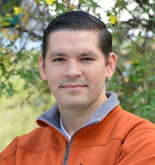
\includegraphics[width=1in,height=1.25in,clip,keepaspectratio]
{img/image001.png}}]{Luis Fernando Gutierrez-Preciado.} received 
his BE degree in Computer Systems from the Autonomous University 
of Aguascalientes, Mexico, in 2007. He obtained his MSc in Computer 
Science and his Ph.D. from CINVESTAV Guadalajara in 2009 and 2013 
respectively. Currently, he is a professor at Western Institute of
Technology and Higher Education in the Department of Electronics,
Systems, and Informatics. His research interests include graph
analytics and self-organizing networks.
\end{IEEEbiography}

\EOD

\end{document}
